\section{Component results and development comparisons}
\label{sec:project-results}
We obtained three kinds of result: learned reductions in native Kira cost, exact shortcuts for specified integral structures, and savings from sharing work between compatible requests. The following comparisons identify the control and workload for each result. Their ratios describe separate experiments and are not factors in a single universal speedup.

\subsection{Seed, equation, and row selection inside Kira}
Using the first seed model with already supplied identities reduced time by 8.6\% on twelve single-target batches: the model-to-full-pool ratio was 0.914, with interval $[0.871,0.958]$. Generating that identity pool was outside this timer. The corresponding sixteen-target comparison had ratio 0.952 with an interval crossing one, so the larger-batch gain was unresolved.

We then placed the learned decisions inside native equation generation and elimination. This test included the work absent from the supplied-equation comparison. The original row model increased complete time by 30.5\% in 84 trials. A later compiled row-cost policy gave ratio 0.982 with interval $[0.959,1.003]$ on sixteen batches from eight physical profiles. Its interval includes equal time. We therefore omitted learned row selection from the retained application.

Equation selection gave a clearer native result. Filtering seed--operator pairs before constructing their coefficients reduced equation-preparation time by 36.2\% and complete time by 5.7\% in the original controlled test. The complete-time ratio was 0.943 with interval $[0.915,0.970]$. A later test on 24 new-index batches gave ratio 0.933 with interval $[0.928,0.940]$, or 6.7\% less complete time. The later retained seed policy gave ratio 0.963 with interval $[0.937,0.984]$ on 32 box batches, or 3.7\% less time. These comparisons support learned selection on their stated inputs, while their different controls prevent addition of the percentages.

Transfer to other graph structures exposed a limit. On nonplanar boxes, pentagons, and boxes with external virtuality, the original equation filter needed recovery and took 25.2\% more time in the first transfer study. Training separate seed and equation trees on those structures removed every first-attempt failure in the new reserved comparison. Their time ratios to native choices were still 1.027 and 1.017, with intervals including one. Learning sufficiency solved one difficulty without establishing a total-time gain.

\subsection{Training for complete cost and the required master basis}
We next trained models on measured reduction cost. The initial common strategy predictor changed time little relative to an equally prepared native control. Separate strategies for seven known graph structures performed better: their aggregate ratio to native choices was 0.937, and the ratio to the per-graph fixed control was 0.944. This second comparison isolates the added request-dependent selection more closely.

Selective seed expansion and reduction through an intermediate master basis then gave a ratio of 0.852 to native choices and 0.926 to the matched fixed strategy on 36 batches. With equal weight for each graph, this corresponds to 14.8\% and 7.4\% less time, respectively. Summed batch medians were 106.24 seconds for native choices and 77.03 seconds for the selected method. The 27.5\% reduction in that sum differs from the 14.8\% equal-graph result because long requests receive more weight in the total. All 720 timed reductions passed the exact comparisons.

We also tested alternative integral orderings, the number of arithmetic threads, wider action portfolios, and models that used structural features rather than family names. The ordering extension did not improve its preceding method. Thread selection improved the preceding method by 1.8\%, but its interval against the matched fixed control included equal time. These tests show why each additional learned choice requires its own comparison.

A portfolio model chooses a complete reduction strategy from a defined set. Our five choices combined earlier policies or selective numerator-rank expansion with one or two Kira workers. Trees selected from 47 training and 26 validation batches were tested on 26 further batches from nine known structures through four loops, including symbolic scattering inputs. Total time was 85.497 seconds against 108.029 seconds for native choices and 86.809 seconds for the per-graph fixed portfolio. The gain against the stronger fixed control was therefore 1.5\%, compared with 20.9\% against native choices.

We then retained those model decisions and reduced repeated symmetry preparation and equation construction around them. On another 26-batch collection, selected-method time fell from 79.784 to 64.183 seconds, a 19.6\% saving from the integration changes. Native choices with the same improved preparation took 87.847 seconds, and the matched fixed portfolio took 67.381 seconds. These controls give savings of 26.9\% and 4.7\%, respectively. All 312 timed reductions passed the exact checks. A fixed portfolio can still contain an earlier learned policy, so this comparison isolates the added outer selection rather than removing every model.

The shared structural model supplies a separate generalization result. It used 44 features and a neural network with two 48-component hidden layers to select among ten seed configurations. On 43 matched native requests, complete time fell from 63.450 seconds for native choices to 57.125 seconds, or 10.0\% less time. The fixed control took 60.094 seconds, so the added learned choice saved 4.9\%. Fifteen matched requests came from excluded physical groups or loop orders; their learned-to-fixed ratio was 0.885. The model and physical inputs are specified in Appendix~\ref{project:app:shared}.

\begin{table}[!htbp]\centering\small
\caption{Selected native comparisons in this study. Each ratio divides the selected method's time by its stated control. Intervals retain the original experiment's paired resampling method; graph-weighted and summed-time estimators are distinct.}
\label{tab:project-ml}
\begin{tabularx}{\linewidth}{@{}YYrr@{}}\toprule
Intervention & Control and estimator & Ratio & Interval\\\midrule
Equation filter, original test & Native; equal physical groups & 0.943 & $[0.915,0.970]$\\
Equation filter, new indices & Native; fixed-request repetitions & 0.933 & $[0.928,0.940]$\\
Graph-specific strategy & Per-graph fixed; equal graphs & 0.944 & $[0.899,0.986]$\\
Selective expansion and basis conversion & Fixed strategy; equal graphs & 0.926 & $[0.876,0.975]$\\
Shared structural model & Global fixed; summed medians & 0.951 & $[0.916,0.971]$\\
Retained box seed policy & Fixed seed region; summed medians & 0.963 & $[0.937,0.984]$\\
Compiled row policy & Native rows; grouped geometric mean & 0.982 & $[0.959,1.003]$\\
Learned choices after reconstruction & Fixed choices; summed medians & 0.983 & $[0.951,1.003]$\\\bottomrule
\end{tabularx}
\end{table}
\begin{figure}[!htbp]\centering
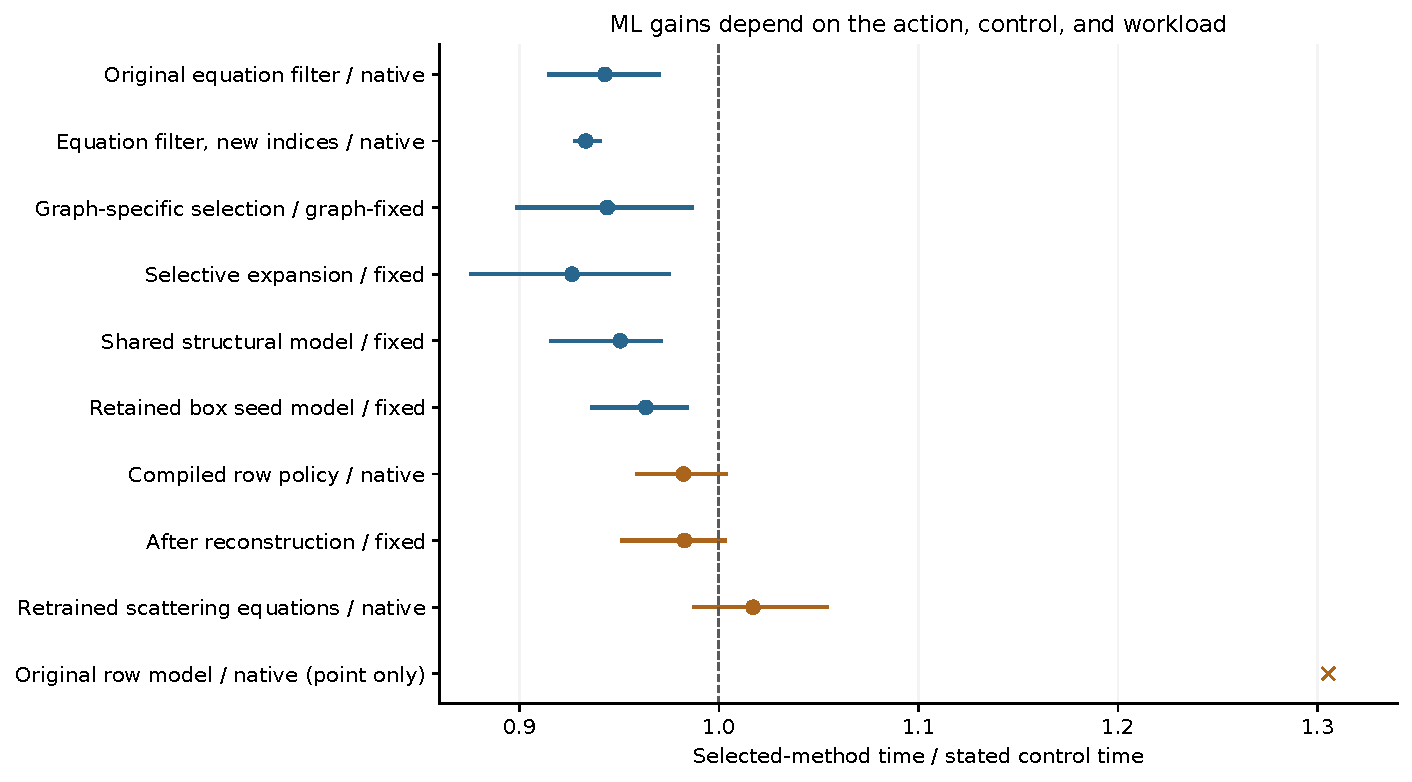
\includegraphics[width=\linewidth]{paper_figures/project_ml.pdf}
\caption{We measured gains from learned choices on some workloads and retained unresolved or slower results. Each point and interval comes from the named experiment and control in Table~\ref{tab:project-ml}. The original row and adapted scattering results are included to show the rejected approaches. The equal-time line is one. These separate comparisons do not form a cumulative sequence.}
\label{fig:project-ml}
\end{figure}
The shared-model grid contained 110 requests, of which only 43 produced a complete matched native comparison. Twenty-one initial references and ten enlarged-region checks failed, and 36 inputs exceeded the tested native coordinate limit. Completed comparisons reached five loops, with only two matched requests at five loops; their aggregate learned-to-native ratio was 1.172. Figure~\ref{fig:project-coverage} keeps the full requested range visible. The 4.9\% learned gain therefore applies to the matched set and does not establish successful acceleration throughout the grid.

\begin{table}[!htbp]\centering\small
\caption{Models we developed and the measured reason to use or omit them. Each row names its own control. The final application retains a validated seed policy, while the other rows report distinct experiments in the study.}
\label{tab:model-study-summary}
\begin{tabularx}{\linewidth}{@{}>{\raggedright\arraybackslash}p{3.4cm}YY@{}}\toprule
Model and representation & Decision and advantage & Measured result and limitation\\\midrule
Seed-set neural classifier; 28,097 parameters & Independent seed probabilities allow several seeds per target; learns from exact construction records & 94.515\% sufficient predicted sets on 690,382 constructed test targets. This accuracy does not establish a native runtime gain\\
Row neural ranker; 10,529 parameters, 132 input features & Scores allowed elimination steps from the current state & 30.5\% slower in 84 native trials. The later compiled cost policy gives ratio 0.982 with interval $[0.959,1.003]$. Omitted\\
Equation decision tree; 17 seed, operator, and target features & Rejects unlikely useful equations before full construction & $72.295\to67.478$ s on 24 new-index batches: 6.7\% less time. Later nonplanar filtering causes recovery on all attempts; disabled in the final test\\
Graph-specific cost trees and strategy selectors & Choose seed enlargement, basis conversion, or a complete strategy from measured time & Selective expansion and basis conversion save 7.4\% against a per-graph fixed choice, with equal graph weighting. Requires training and validation for the tested structures\\
Shared structural neural regressor; 44 inputs, two 48-component layers & Predicts ten seed-action costs without a family-name input & $60.094\to57.125$ s against a global fixed choice: 4.9\% less time on 43 matched requests. Some classes are slower; Table~\ref{tab:native-type-summary} gives every class\\
Native seed-cost trees with failure checks & Choose a seed region, or use a conservative fixed action when risk is high & Earlier 32-box test: $156.383\to150.663$ s, 3.7\% less than fixed seeds. Later 24-box test: $200.983\to198.313$ s, 1.3\% less, with interval including equal time\\
Tensor-order cost tree and later arithmetic forests & Attempt to choose an exact recurrence order or native arithmetic setting & Validation did not justify deployment; final methods use fixed choices. Exact-method gains are reported separately\\\bottomrule
\end{tabularx}
\end{table}

\subsection{The large cumulative gain from exact vacuum recurrences}
\label{sec:project-vacuum-results}
The constructed high-loop data also led to a mathematical shortcut. In the restricted coupled-vacuum family, every massive denominator depends on the same momentum sum, and all massless lines have power one. Euler identities and mass partial fractions reduce every accepted target to one-power masters. Their coefficients depend on the loop order through the single variable $z=L(d-2)$, so one exact polynomial calculation serves several loop orders. Appendix~\ref{app:project-vacuum} derives the recurrence and an independent Taylor partial-fraction check.

We tested the cumulative change directly against the original saved Kira 3.1 executable on eight new groups, each with three mass profiles and all loop orders one through twelve. Both baseline arms constructed the complete supplied Euler and mass-identity systems for each mass profile and loop order. The exact method used the fixed recurrence, shared loop dependence, and exact coefficient expansion. A learned recurrence selector was trained and tested, but the final validation-selected rule was fixed. Thus this large gain is an exact-method and work-sharing result.

Summing one complete-time median per group gives 1,027.781 seconds for the original baseline and 1.922 seconds for the exact method, a 534.9-fold speedup. The equally weighted geometric mean of the eight speedups is 543.8, with descriptive interval $[488.1,605.1]$. Both measures include fresh-process startup, input preparation, equation construction where required, exact algebra, checking, and output writing and reading. All 120 workflows complete; each baseline arm makes 1,440 Kira calls over its repetitions, while the successful exact arm makes none. Independent checks cover 27,960 nonzero coefficient polynomials.

\begin{figure}[!htbp]\centering
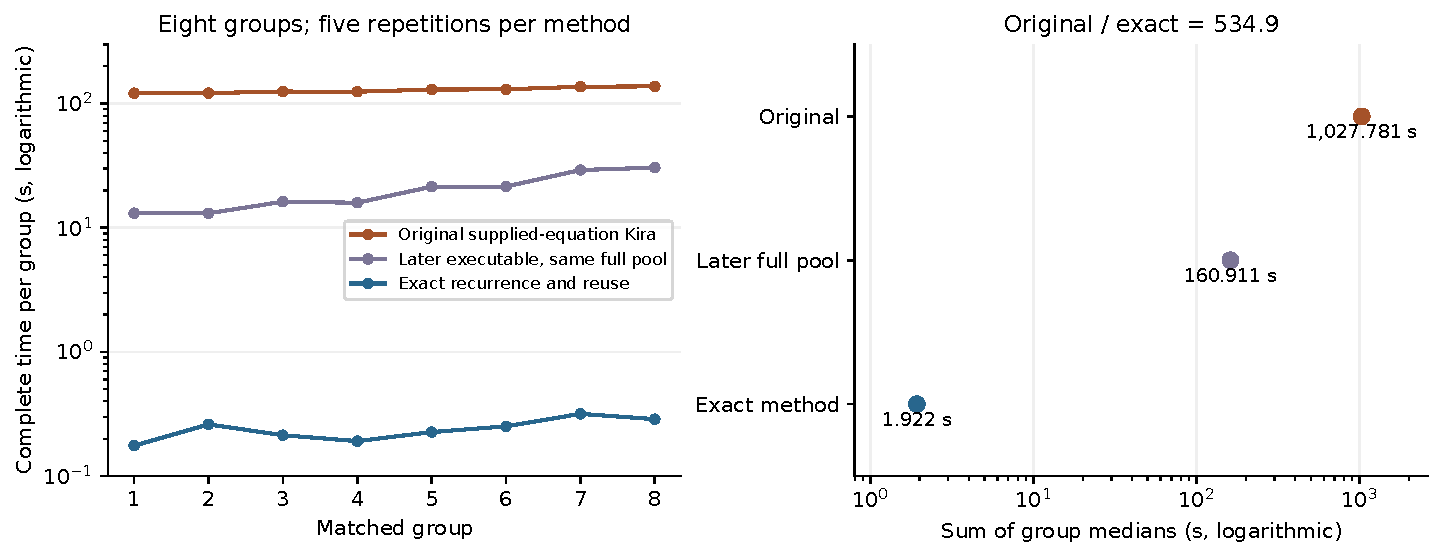
\includegraphics[width=\linewidth]{paper_figures/project_cumulative.pdf}
\caption{A direct original-to-optimized comparison for the restricted vacuum family. Left: median complete time for each of eight matched groups on a logarithmic axis. Each group contains three mass profiles and loop orders one through twelve. Right: sums of group medians, also on a logarithmic axis. The original and later executable controls solve supplied identities separately; the exact recurrence shares their symbolic solution. The 534.9-fold total-time ratio is not a model-only gain or a result for general scattering.}
\label{fig:project-cumulative}
\end{figure}

\subsection{Sharing requests and extending the analytic domains}
Another saving comes from combining target lists that have identical family definitions and kinematics. On ten compatible request groups, joint reduction with native choices and the common implementation had ratio 0.517 to separate native reductions, with interval $[0.507,0.535]$: 48.3\% less time. Adding the learned choice gave ratio 0.996 against that joint fixed control, with an interval crossing one. Linearity permits the shared answer to be separated back into the original requests, as derived in Appendix~\ref{app:project-construction}.

We also separated independent loop blocks, reused exact component reductions, and replaced suitable native calculations by analytic identities. The resulting domains include massless and one-mass two-point structures, connected bubble trees, one-loop tensor numerators, zero-invariant bubbles, vacuum partial fractions, and massless triangles. We derived their conditions before applying them, and tested restricted connected trees and independent products through thirteen loops. These additions are summarized in Table~\ref{tab:exact-domains}; their derivations remain in the appendices.

The development included compact basis preparation, failure-aware choices, basis-compatible seed bounds, symbolic factorization, cancellation of Gamma factors, and delayed model loading. Each change addressed a measured cost. For example, compact preparation without ML had ratio 0.305 to expanded discovery on thirteen matched requests, while the added neural choice had ratio 0.982 to the compact fixed procedure on 22 requests and did not resolve an additional gain. In another complete-cost experiment, the method completed 126 of 127 requests and saved 6.0\% against the preceding application, but gave no resolved extra gain against the matched fixed control. These outcomes prevented setup savings and successful recovery from being reported as model-only acceleration.

\subsection{Secondary combined results and application updates}
\label{sec:project-combined}
Table~\ref{tab:project-overall} collects complete-time results whose baselines were measured directly. They answer different practical questions: repeated reductions of an analytically reducible family, compatible requests that can share a system, a native model choosing a seed configuration, and mixed analytic/native workloads.

\begin{table}[!htbp]\centering\small
\caption{Secondary comparisons with explicit controls. These historical component and development tests do not replace the default-Kira comparison in Table~\ref{tab:default-kira-final}. Each row is a separate matched experiment. Times are sums of request or group medians, except the final row, which uses the median time of a complete collection. No row combines percentages from different tests.}
\label{tab:project-overall}
\begin{tabularx}{\linewidth}{@{}YrrY@{}}\toprule
Workload and control & Control (s) & Method (s) & Measured gain\\\midrule
Restricted vacuum; original supplied-equation Kira & 1,027.781 & 1.922 & 534.9-fold; exact recurrence and reuse\\
36 native batches; native choices & 106.24 & 77.03 & 27.5\% less total time; selective expansion and basis conversion\\
26 native batches; equally prepared native choices & 87.847 & 64.183 & 26.9\% less; integrated strategy portfolio\\
Same 26 batches; fixed portfolio & 67.381 & 64.183 & 4.7\% less; added outer selection\\
43 native requests; global fixed choice & 60.094 & 57.125 & 4.9\% less; shared learned choice\\
75 mixed requests; before direct vacuum and reconstruction additions & 81.827 & 49.852 & 39.1\% less; combined additions\\
93 mixed requests; preceding integrated application & 45.091 & 41.137 & 8.8\% less; final update\\\bottomrule
\end{tabularx}
\end{table}
On the 75-request collection, enabling the validated finite-field reconstruction settings reduced time from 79.624 to 49.852 seconds, or 37.4\%. Comparing the same final result directly with the application before both the direct-vacuum and reconstruction additions gives 81.827 to 49.852 seconds, or 39.1\%. Those are matched comparisons on the same collection; they are the relevant cumulative measurements for that stage.

The later 93-request study gives the additional 8.8\% reduction from 45.091 to 41.137 seconds. It contains 20 native and 73 analytic requests and checks all 837 outputs from three methods and three repetitions. This is the last incremental comparison, rather than the overall outcome of the study. Appendix~\ref{app:latest-results} retains its full timing tables, three plots, subgroup regressions, and failed parallel predecessor.

The final application combines admitted exact identities, shared work, the inherited validated seed model, and fixed native arithmetic choices. The original row model remains omitted. The latest arithmetic selector failed its validation condition, and the added nonplanar equation filter was 71.1\% slower after recovery; both remain disabled. In the reconstruction-era model-only comparison, the ratio to fixed choices was 0.983 with interval $[0.951,1.003]$, so a reliable extra aggregate ML gain was unresolved. Earlier positive model results remain valid for their own tests; they do not make every later configuration faster.

\begin{figure}[!htbp]\centering
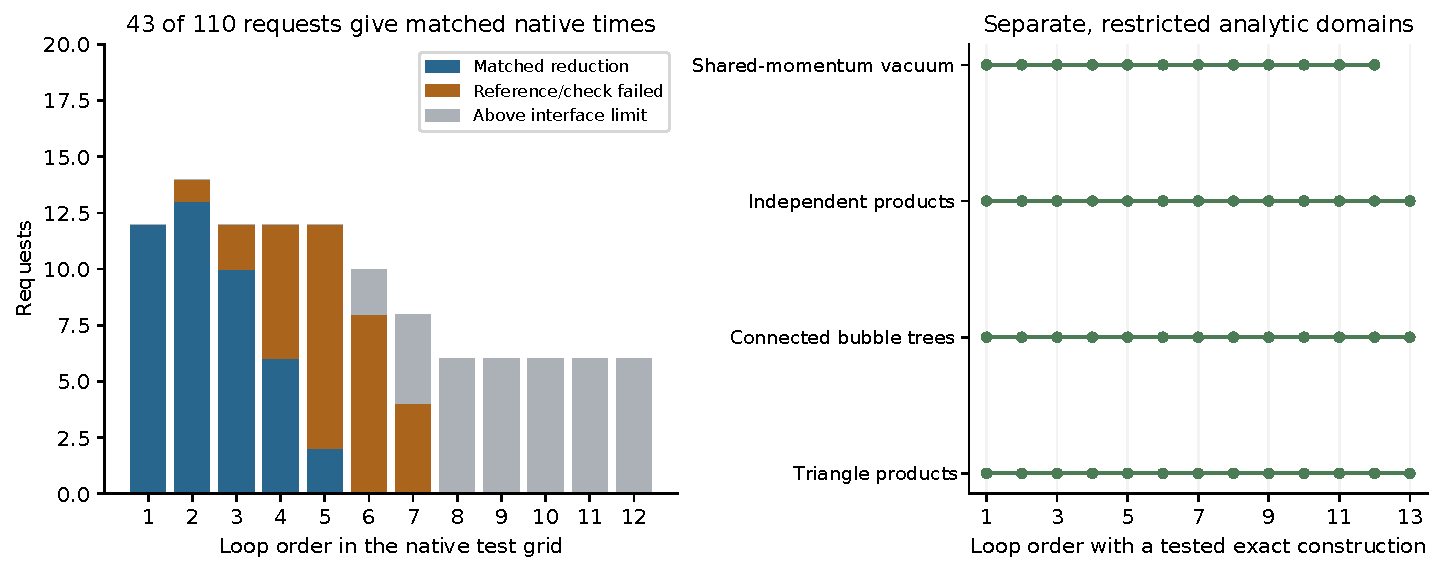
\includegraphics[width=\linewidth]{paper_figures/project_coverage.pdf}
\caption{Loop count and mathematical structure define different limits. Left: all 110 requests in the shared-model native test, including failed reference checks and inputs above the tested interface's coordinate limit. Right: the loop ranges demonstrated by selected exact constructions in separate studies. The higher-loop analytic results concern the stated restricted structures, not all connected graphs. No native timing at loop orders six through twelve is inferred from an analytic result.}
\label{fig:project-coverage}
\end{figure}
\FloatBarrier
